\section{Post-Training}

The post-training phase of GLM-5 aims to transform the base model into a highly capable assistant with robust reasoning, coding, and agentic abilities. As illustrated in Figure~\ref{fig:overall_pipeline}, our pipeline follows a progressive alignment strategy: starting with multi-task Supervised Fine-Tuning (SFT) that introduces sophisticated interleaved thinking modes, followed by specialized Reinforcement Learning (RL) stages for reasoning and agentic tasks, and concluding with a general RL stage for human-style alignment. By leveraging on-policy cross-stage distillation as the final refinement, GLM-5 effectively mitigates capability regression while harnessing the performance gains from each training stage.

\subsection{Supervised Fine-Tuning}

\begin{figure}[!t]
    \centering
    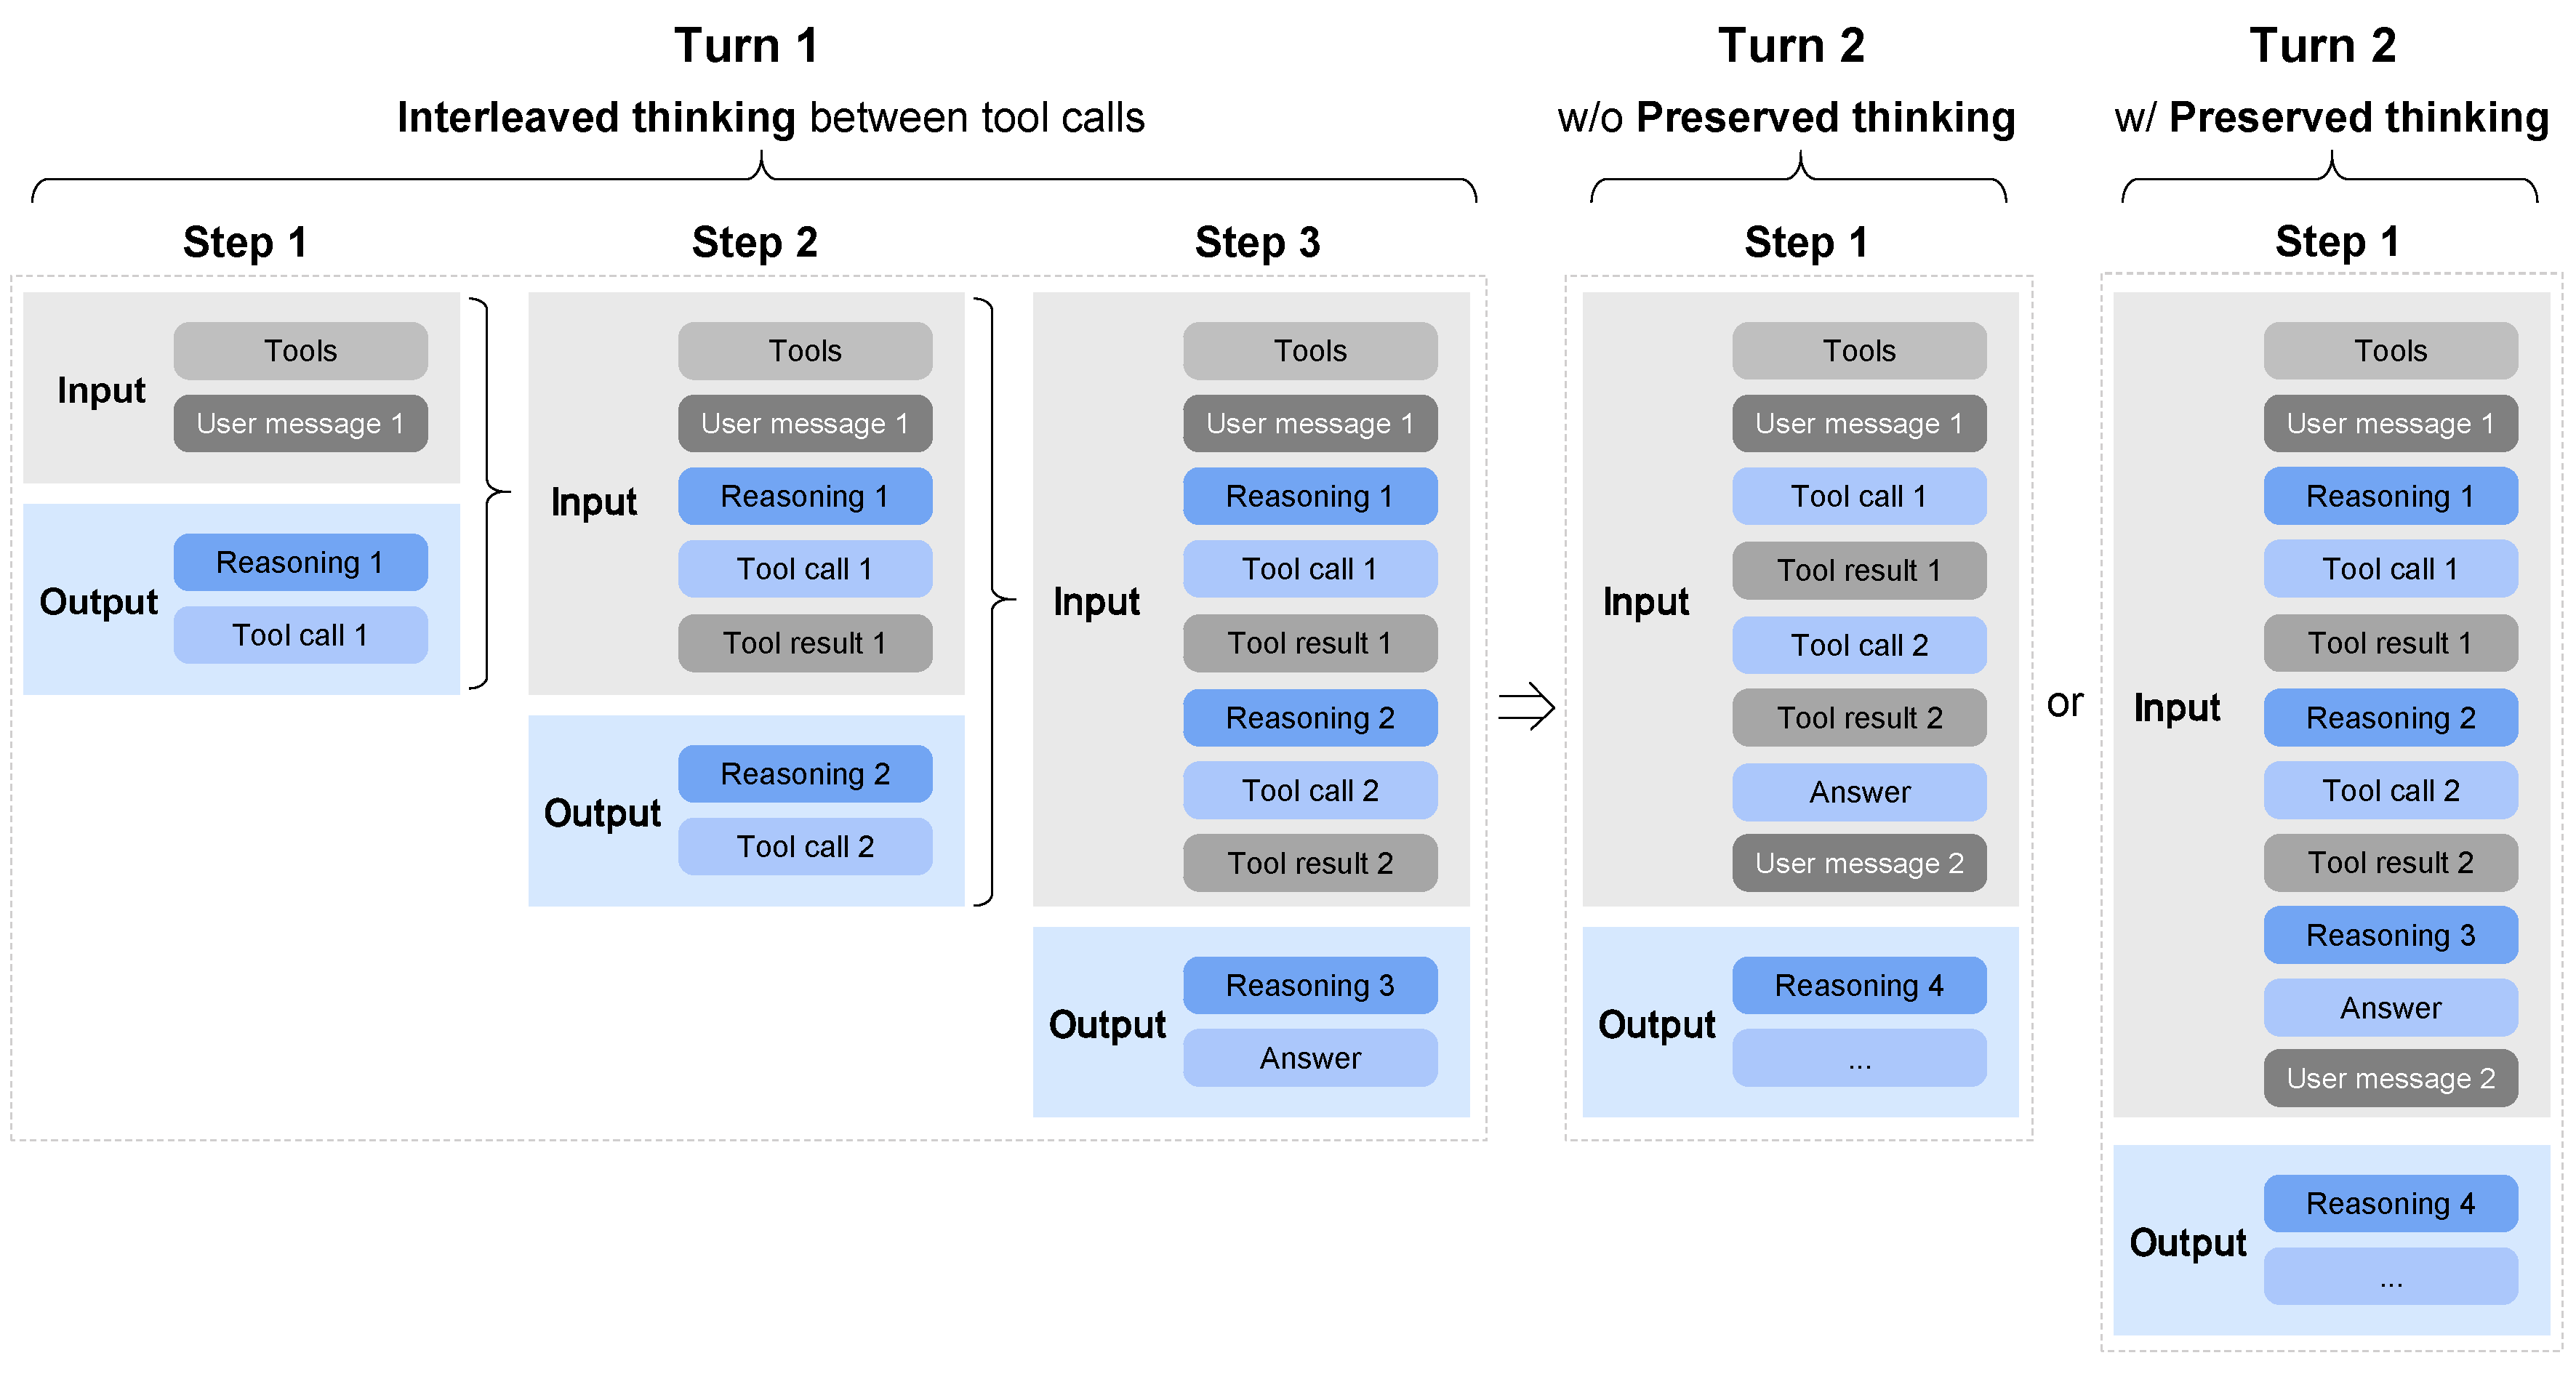
\includegraphics[width=\linewidth]{figures/glm5_tr_thinking_mode_v2.pdf}
    \caption{Illustration of Interleaved Thinking and Preserved Thinking.}
    \label{fig:thinking_mode}
\end{figure}

Compared with GLM-4.5, GLM-5 significantly expands the scale of \emph{Agent} and \emph{Coding} data during the SFT stage. The SFT corpus of GLM-5 covers three major categories:
\begin{itemize}[leftmargin=1.5em,itemsep=2pt]
    \item \textbf{General Chat}: question answering, writing, role-playing, translation, multi-turn dialogue, and long-context interactions;
    \item \textbf{Reasoning}: mathematical, programming, and scientific reasoning;
    \item \textbf{Coding \& Agent}: frontend and backend engineering code, tool calling, coding agents, search agents, and general-purpose agents.
\end{itemize}

Additionally, GLM-5 extends the maximum context length to 202,752 tokens during SFT. Along with an updated chat template, the model supports three distinct thinking characteristics (see Figure \ref{fig:thinking_mode}), including:


\begin{itemize}[leftmargin=1.5em,itemsep=2pt]
    \item \textbf{Interleaved Thinking}: the model thinks before every response and tool call, improving instruction following and the quality of generation\footnote{Interleaved thinking was first introduced by \url{https://platform.claude.com/docs/en/build-with-claude/extended-thinking\#interleaved-thinking}}.
    \item \textbf{Preserved Thinking}: in coding agent scenarios, the model automatically retains all thinking blocks across multi-turn conversations, reusing existing reasoning instead of re-deriving it from scratch. This reduces information loss and inconsistencies, and is well-suited for long-horizon, complex tasks\footnote{Preserved thinking was also adopted by Claude since Opus 4.5. See \url{https://platform.claude.com/docs/en/build-with-claude/extended-thinking\#thinking-block-preservation-in-claude-opus-4-5-and-later}}.
    \item \textbf{Turn-level Thinking}: the model supports per-turn control over reasoning within a session—disable thinking for lightweight requests to reduce latency/cost, enable it for complex tasks to improve accuracy and stability.
\end{itemize}

By thinking between actions and maintaining consistency across turns, GLM-5 achieves more stable and controllable behavior on complex tasks.

For \textbf{General Chat}, we optimize the response style to be more logical and concise compared to GLM-4.5. For role-playing tasks, we collect and construct a broader and more diverse dataset covering multiple languages and role configurations. In particular, we define several evaluation dimensions---including instruction following, linguistic expressiveness, creativity, logical coherence, and long-dialogue consistency---and apply both automatic and human filtering to curate and refine the data.

For \textbf{Reasoning} tasks, we further enhance the depth of the model's reasoning. Specifically, for logical reasoning, we construct verifiable problems and synthesize high-quality data using rejection sampling. For mathematical and scientific problems, a difficulty-based filtering process is applied, retaining only problems that are challenging for the GLM-4.7 model.

For \textbf{Coding} and \textbf{Agent} tasks, compared to GLM-4.5, GLM-5 constructs a large number of execution environments to obtain high-quality trajectories, with particular emphasis on real-world scenarios and long-horizon tasks. We further improve the SFT data using expert reinforcement learning and rejection sampling. Erroneous segments within trajectories are retained but masked out in the loss function, allowing the model to learn error correction behaviors without reinforcing incorrect actions.

\subsection{Reasoning RL}

\paragraph{RL algorithm backbone.}
Our RL algorithm builds upon GRPO~\cite{shao2024deepseekmath} and incorporates the IcePop technique~\cite{IcePop2025} to mitigate the \emph{training-inference mismatch}, i.e., the discrepancy between the inference distribution and the training distribution during RL optimization. We explicitly distinguish between the \emph{training policy} $\pi^{\text{train}}$, used for gradient updates, and the \emph{inference policy} $\pi^{\text{infer}}$, used for trajectory sampling. Compared to the original IcePop formulation, we remove the KL regularization term to accelerate RL improvement.
The final optimization loss is:
\begin{equation}
\begin{aligned}
\mathcal{L}(\theta)=
-\mathbb{E}_{
x \sim \mathcal{D},
\{y_i\}_{i=1}^{G} \sim \pi^{\text{infer}}_{\theta_{\text{old}}}(\cdot \mid x)
}
&\Bigg[
\frac{1}{G}
\sum_{i=1}^{G}
\frac{1}{|y_i|}
\sum_{t=1}^{|y_i|}
\operatorname{pop}
(\rho_{i,t}, 1/\beta, \beta) \\
&\cdot
\min\!\left(
r_{i,t}\hat{A}_{i,t},
\operatorname{clip}\!\left(
r_{i,t},
1-\epsilon_{\text{low}},
1+\epsilon_{\text{high}}
\right)
\hat{A}_{i,t}
\right)
\Bigg],
\label{icepop}
\end{aligned}
\end{equation}
where the training-inference mismatch ratio is defined as
\begin{align*}
\rho_{i,t}
=
\frac{
\pi_{\theta_{\text{old}}}^{\text{train}}(y_{i,t} \mid x, y_{i,<t})
}{
\pi_{\theta_{\text{old}}}^{\text{infer}}(y_{i,t} \mid x, y_{i,<t})
}.
\end{align*}

The operator $\operatorname{pop}(\cdot)$ suppresses samples whose mismatch ratio deviates excessively:
\begin{align*}
\operatorname{pop}(\rho_{i,t}, 1/\beta, \beta)
=
\begin{cases}
\rho_{i,t}, & 1/\beta \le \rho_{i,t} \le \beta, \\
0, & \text{otherwise}.
\end{cases}
\end{align*}

The PPO-style importance ratio and the group-normalized advantage follow the original GRPO definition:
\begin{align*}
r_{i,t}
=
\frac{
\pi_\theta^{\text{train}}(y_{i,t}\mid x,y_{i,<t})
}{
\pi_{\theta_{\text{old}}}^{\text{train}}(y_{i,t}\mid x,y_{i,<t})
},
\quad
\hat{A}_{i,t}
=
\frac{
R_i - \operatorname{mean}(R_1,\dots,R_G)
}{
\operatorname{std}(R_1,\dots,R_G)
}.
\end{align*}

During training, we set hyperparameters $\beta=2, \epsilon_{\text{low}}=0.2, \epsilon_{\text{high}}=0.28$. Training is performed entirely on-policy with a group size of 32 and a batch size of 32.

\paragraph{DSA RL insights.}
We conduct a very large-scale RL training on a model based on the DSA architecture. Compared with MLA, DSA introduces an additional indexer that retrieves the top-k most relevant key-value entries and computes attention sparsely over the retrieved subset.
The retrieved top-k results are critical for RL stability. This is analogous to how MoE models use routing replay~\cite{zheng2025group} to preserve the activated top-k experts to ensure training-inference consistency.
However, directly adapting this strategy to indexer replay, i.e., storing the indexer’s top-k indices at every token position is clearly impractical, since the $k = 2048$ used by the indexer is much larger than the $k$ typically used in MoE, and storing all these indices would incur enormous storage costs as well as significant communication overhead between the training engine and the inference engine.

We find that adopting a deterministic top-k operator effectively resolves the training-inference mismatch in DSA indexer token selection. Compared with the non-deterministic CUDA-based top‑k implementation used in SGLang’s DSA Indexer, directly using the naive \texttt{torch.topk} is slightly slower but deterministic. It produces more consistent outputs and yields substantial RL gains. In contrast, other non-deterministic top‑k operators (e.g., CUDA or TileLang implementations) caused drastic performance degradation during RL after only a few steps, accompanied by a sharp drop in entropy. Therefore, throughout our RL stages, we use \texttt{torch.topk} as the default top-k operator in the DSA Indexer in our training engine. We also freeze the indexer parameters by default during RL to accelerate training and prevent unstable learning in the indexer.

\paragraph{Mixed domain reasoning RL.} In the Reasoning RL stage, we perform mixed RL training over four domains: mathematics, science, code, and tool-integrated reasoning (TIR). For mathematics and science, we curate data from both open-source datasets~\cite{du2025nemotron, moshkov2025aimo} and co-developed collections with external annotation vendors. We further apply difficulty filtering to focus training on problems that GLM-4.7 solves correctly only rarely or fails consistently, while remaining solvable by stronger teacher models (e.g., GPT-5.2 xhigh and Gemini 3 Pro Preview). For code, we cover both competitive programming style tasks and scientific coding tasks. The former is primarily sourced from Codeforces and representative datasets such as TACO~\cite{li2023taco} and SYNTHETIC-2-RL~\cite{synthetic2_blog_2025}, while the latter is constructed from internal problem pools by decomposing questions into the minimal code implementations required for correct solutions. For TIR, we reuse the more challenging subset of mathematics and science RL data, and additionally co-build STEM questions with annotation vendors that are explicitly designed to be answered with external tools. During RL training, we assign domain and source-specific judge models or evaluation systems to produce binary outcome rewards. We keep the overall mixture roughly balanced across the four domains, and consistently observe stable and significant gains in each domain under the mixed RL setting.

\subsection{Agentic RL}
To facilitate agentic performance of GLM-5, we develop a fully asynchronous and decoupled RL framework and optimize GLM-5 in coding and search agent tasks. Naive synchronous RL suffers from severe GPU idle time during long-horizon agent rollouts. By decoupling inference and training engines via a central Multi-Task Rollout Orchestrator, we achieve high-throughput joint training across diverse agentic workloads.

To maintain training stability under asynchronous off-policy conditions, we introduce two key mechanisms. First, a Token-in-Token-out (TITO) gateway eliminates re-tokenization mismatches by preserving exact action-level correspondence. Second, we employ a Direct Double-sided Importance Sampling, which applies a token-level clipping mechanism ($[1-\epsilon_\ell, 1+\epsilon_h]$) to rollout log-probabilities, while efficiently controlling off-policy bias without tracking historical policy checkpoints. We also employ a DP-aware routing to maximize KV-cache reuse during long-context inference for large-scale MoE models for speed up. To scaling agentic environments, we scale verifiable training environments across three domains: over 10K real-world Software Engineering (SWE), terminal tasks, and high-difficulty multi-hop search tasks. More details about agentic RL can be found in the subsequent Section 4.

\subsection{General RL}

\paragraph{Multi-dimensional optimization objectives.}
We decompose the optimization objectives of General RL into three complementary dimensions: \emph{foundational correctness}, \emph{emotional intelligence}, and \emph{task-specific quality}.

The \emph{foundational correctness} dimension serves as the bedrock of response quality. It targets a broad spectrum of error types that undermine the usability of model outputs, including instruction-following failures, logical inconsistencies, factual inaccuracies, knowledge hallucinations, and language disfluencies. The goal is to minimize the error rate so that responses reach a \emph{usable} baseline. We consider this a prerequisite for all subsequent optimization: a response containing factual errors or misinterpreting the user's intent can actively mislead the user, no matter how polished it may appear.

The \emph{emotional intelligence} dimension optimizes user experience beyond core correctness. It aims to produce responses that are empathetic, insightful, and stylistically close to natural human communication, making interactions with the model feel more natural and engaging.

The \emph{task-specific quality} dimension targets fine-grained optimization across various specific tasks. Building on the usability established by foundational correctness, it aims to elevate responses from merely correct to genuinely high-quality within each task category. This dimension covers a wide range of tasks, including writing, text processing, subjective and objective question answering, role-playing, and translation. Each task domain demands distinct reward signals, necessitating a hybrid reward system.

\paragraph{Hybrid reward system.}
To supervise the diverse objectives above, we build a hybrid reward system that integrates three complementary types of reward signals: \emph{rule-based reward functions}, \emph{outcome reward models} (ORMs), and \emph{generative reward models} (GRMs). Each has distinct strengths and weaknesses, and their combination is key to a stable, efficient, and scalable General RL training process.

Rule-based rewards provide precise and interpretable signals, but are limited to aspects expressible as deterministic rules. ORMs offer low-variance signals and high training efficiency, but are more susceptible to reward hacking, where the policy exploits superficial patterns rather than genuinely improving core capability. GRMs leverage language models to produce scalar or structured evaluations and are more robust to such exploitation, but tend to exhibit higher variance. By blending these three signal types, we obtain a reward system that balances precision, efficiency, and robustness, mitigating the weaknesses of any single component.

\paragraph{Human-in-the-loop style alignment.}
A distinctive aspect of our General RL pipeline is the explicit incorporation of high-quality human-authored responses. Rather than relying solely on model-generated responses, we introduce expert human responses as stylistic and qualitative anchors. This is motivated by the observation that purely model-generated optimization tends to converge toward recognizably ``model-like'' patterns---often verbose, formulaic, or lacking the nuance of skilled human writing. By exposing the model to human-written exemplars, we encourage it to adopt more natural, human-aligned response patterns.

\subsection{On-Policy Cross-Stage Distillation}
In our multi-stage RL pipeline, sequentially optimizing for distinct objectives can lead to the cumulative degradation of previously acquired capabilities. To mitigate this issue, we perform on-policy cross-stage distillation as the \textbf{final stage}, adopting an on-policy distillation algorithm~\cite{guminillm,qwen3,xiao2026mimov2flashtechnicalreport,lu2025onpolicydistillation} to swiftly recover the skills acquired in earlier SFT and RL stages (Reasoning RL and General RL). Specifically, the final checkpoints from the preceding training stages serve as teacher models, where the training prompts are sampled from the corresponding teachers' RL training sets and mixed in appropriate proportions. The training loss can be obtained by replacing the advantage term in Eq.~\ref{icepop} with the following formula (`sg' stands for the stop gradient operation, e.g., \texttt{.detach()}):

\begin{equation}
    \hat{A}_{i,t} = \text{sg}\left[\log\frac{\pi_{\theta_{\text{teacher}}}^{\text{infer}}(y_{i,t}\mid x,y_{i,<t})}{\pi_\theta^{\text{train}}(y_{i,t}\mid x,y_{i,<t})}\right].
\end{equation}

Currently, we utilize the inference engine to fetch teachers' logits. In the future, we plan to migrate the inference backend to the training engine and uniformly adopt the Multi-Query Attention (MQA) mode of MLA for inference ($\pi_{\theta_{\text{teacher}}}^{\text{infer}}\rightarrow\pi_{\theta_{\text{teacher}}}^{\text{train}}$).
During training, the group size in the GRPO algorithm is configured to 1 to increase data throughput, and the batch size is set to 1024. This is feasible at this stage because it is no longer necessary to maintain a large group of samples per prompt to estimate advantages; the advantage is computed directly from the gap with the teacher models instead.

\subsection{RL Training Infrastructure: The \emph{slime} Framework}

We continue to use slime as the unified post-training infrastructure for GLM-5, enabling end-to-end reinforcement learning (RL) at scale. Rather than introducing new system components, GLM-5 \emph{fully leverages} slime's capabilities to (1) broaden task coverage via free-form rollout customization and a server-based execution model, (2) substantially increase throughput via mixed-precision training/rollouts together with MTP and Prefill-Decode (PD) disaggregation---particularly for multi-turn RL workloads, and (3) improve robustness through heartbeat-driven rollout fault tolerance and router-level server lifecycle management.

\subsubsection{Scaling Out: Flexible Training via Highly Customizable Rollouts}
GLM-5’s post-training spans a diverse spectrum of objectives. To support this diversity without task-specific forks, GLM-5 leverages slime's highly customizable rollout interface together with its server-based rollout execution.

\textbf{Highly customizable rollouts.} slime provides a flexible interface for implementing task-specific rollout logic---including multi-turn interaction loops, tool invocation, environment feedback handling, and verifier-guided branching---without modifying the underlying infrastructure. GLM-5 leverages this capability to support a broad range of domains and training paradigms, including but not limited to reasoning RL, general RL, agentic RL, and on-policy distillation, all within a unified training stack.

\textbf{Server-based rollouts via HTTP APIs.} slime exposes its rollout servers and inference router through standard HTTP APIs, allowing users to interact with slime's serving layer in the same way as a conventional inference engine. This decouples rollout logic from the training process boundary: external agent frameworks and environments can call the server/router endpoints directly, while the optimization backend remains unchanged for both short-horizon single-turn training and long-horizon multi-turn trajectories.

\subsubsection{Scaling Up: Tail-Latency Optimization for RL Rollouts}
For RL rollouts, the optimization target is not aggregate throughput but \emph{end-to-end latency}, dominated by the slowest (long-tail) sample in each step. In practice, a single straggling trajectory can stall synchronization points (e.g., batch completion, buffer readiness, trainer updates) and directly determine wall-clock progress. GLM-5 therefore fully leverages slime's latency-oriented serving and scheduling mechanisms to minimize both median latency and, more importantly, tail latency.

\textbf{No-queue serving via multi-node inference with DP-attention for MLA.}
To avoid queueing delays, rollout requests must be served promptly even under bursty traffic, which requires substantial KV-cache capacity. GLM-5 adopts a multi-node inference deployment (e.g., EP64 and DP64 over 8 nodes) to provision sufficient distributed KV-cache. DP-attention is primarily introduced to prevent copying KV across different ranks.

\textbf{Tail-latency reduction with FP8 rollouts and MTP.}
GLM-5 uses FP8 for rollout inference to reduce per-token latency and shorten the completion time of long trajectories. In addition, GLM-5 leverages slime's support for Multi-Token Prediction (MTP), which is especially effective under the small-batch decoding regime typical in RL rollouts. Since tail latency is often driven by small-BS stragglers (e.g., rare long contexts, complex multi-turn reasoning, tool-heavy traces), MTP provides disproportionately large benefits on the long tail, improving the time-to-completion of the slowest sample and thus reducing step-level stall time.

\textbf{PD disaggregation to prevent prefill-decode interference in multi-turn RL.}
In multi-turn settings, long-prefix prefills are frequent (conversation history, tool traces, code context). Under DP-attention, mixing prefill and decode on the same serving resources can create severe interference: a heavy prefill can preempt or disrupt ongoing decodes on the server, preventing other samples from making continuous progress and sharply worsening tail latency. GLM-5, therefore, leverages slime's Prefill--Decode (PD) disaggregation. By running prefills and decodes on dedicated resources, decodes remain stable and uninterrupted, enabling long-horizon samples to progress continuously and significantly improving tail behavior in multi-turn agentic RL.

\subsubsection{Rollout Robustness: Heartbeat-Driven Fault Tolerance}

At scale, transient failures (e.g., individual server crashes, network issues, or performance degradation) are inevitable. GLM-5 leverages slime's heartbeat-driven fault-tolerance to ensure training continuity under such events: rollout servers periodically emit heartbeats monitored by the orchestration layer, and unhealthy servers are proactively terminated and deregistered from the inference router. As a result, retries are automatically routed away from failed or degraded servers to healthy ones, preventing single-server incidents from interrupting rollouts and preserving uninterrupted end-to-end RL training.
